\documentclass[12pt]{article}

% Basic stuff
\usepackage{fullpage}
\usepackage{graphicx}
\usepackage[parfill]{parskip}
\usepackage[utf8]{inputenc}

% Skip one line between paragraphs
\parskip1em
 
% Standard things to include for math   
\usepackage{amsmath,amssymb,amsfonts,amsthm}

% Other stuff
\usepackage{hyperref}
\usepackage{datetime} \usdate
\usepackage{enumitem}
\usepackage{changepage}
\usepackage{tcolorbox}


% Some of Ebrahim's definitions
\newcommand{\note}[1]{[#1]}
\newcommand{\done}{\\\hspace*{0pt}\hfill$\blacksquare$}
\def\N{\mathbb{N}}
\def\R{\mathbb{R}}
\def\Q{\mathbb{Q}}
\def\Z{\mathbb{Z}}
\def\e{\varepsilon}
\def\d{\delta}
\newcommand{\seq}[1]{\left(#1\right)_{n\in\N}}
\newcommand{\settext}[2]{\left\{ #1\ |\ \text{#2} \right\}}
\renewcommand{\emptyset}{\{\hspace{-2pt}\}}
\newcommand{\powerset}[1]{\mathcal{P}(#1)}
\newcommand{\dom}[1]{\operatorname{dom}(#1)}
\newcommand{\ran}[1]{\operatorname{ran}(#1)}
\newcommand{\rev}[1]{(#1)^{\dashv}}
\newcommand{\injrightarrow}{\xrightarrow{\text{inj}}}
\newcommand{\surjrightarrow}{\xrightarrow{\text{surj}}}
\newcommand{\bijrightarrow}{\xrightarrow{\text{bij}}}
\newcommand{\AND}{\wedge}
\newcommand{\OR}{\vee}
\newcommand{\ARR}{\Longrightarrow}
\newcommand{\DARR}{\Longleftrightarrow}
\newcommand{\ex}[1]{\textbf{Exercise:}\begin{adjustwidth}{2em}{}#1\end{adjustwidth}}
\newcommand{\indented}[1]{\begin{adjustwidth}{1em}{}#1\end{adjustwidth}}

\newcommand{\THM}[2]{\textbf{Theorem:} #1\\[0.5em]\textit{Proof:} #2\qed}

\newcommand{\RULE}[2]{\begin{tcolorbox}[title=Rule: #1,colbacktitle=white,coltitle=black,colback=white]#2\end{tcolorbox}}
\newcommand{\DRULE}[2]{\begin{tcolorbox}[title=Rule: #1,colbacktitle=white,coltitle=black,colback=white]#2\end{tcolorbox}} % IDK if derived rules will be different

\def\pA{\Phi}
\def\pB{\Psi}
\def\pC{\Omega}
\def\pD{\Sigma}
\def\pE{\Gamma}
\def\pF{\Delta}




\begin{document}

\begin{center} {\Large \scshape Mathematical Proofs and Mathematical Writing}
\end{center}
(compiled on \today\ at\ \currenttime)
\hfill

\tableofcontents

\section{Introduction}

\note{what to put here:
this course is about both set theory and writing.
set theory is axiomatic. describe what i mean by that, why we would do that, and the historical relevance of it.
why rigor anyway?
logic can also be done this way, but we will not.
we will follow a more intuitive and informal writing-focused approach for logic,
saving our rigor-enegery for set theory.
perhaps include a discussion levels of rigor and formality, with one level relegating the rigor to other levels.
mention the importance of writing and the roughness of this transition for many people.
mention the value of forgetting what you knew before, but not really forgetting it all.}

\note{Write the general intro later, maybe last.}



\section{Mathematical Language}
\label{sec:logic}

This section will develop mathematical logic and show you how logical arguments factor into writing.
We do not yet have anything to argue \emph{about}, so our ``proofs'' will be about nothing in particular.
Section \ref{sec:sets} will later give some mathematical objects to talk about, and we will then put
content into the empty skeleton arguments of this section.

\subsection{Parts of Speech}

In a language, a \emph{part of speech} is a collection of words that share grammatical properties.
For example here are some common English parts of speech: pronouns, nouns, verbs, adjectives, and adverbs.
Different languages can have different parts of speech that are useful for describing their grammar.
To build up the grammar of a language, one can specify how parts of speech fit together to form larger
\emph{constituents}, such as noun phrases and clauses. One can further describe how
constituents fit together to form even more complex constituents, eventually grammatical sentences.

Mathematics is a language, and so it makes sense to build up its grammar (its \emph{syntax}) using this same strategy.
Instead of pronouns, nouns, verbs, noun phrases, sentences, and so on, there are just four constitutuents in
mathematics. Two are basic parts of speech and two are more complex constituents:
\begin{itemize}
\item \emph{Variables} are a basic part of speech.
\item \emph{Constants} are a basic part of speech.
\item \emph{Terms} can be built out of variables, constants, other terms, and propositions.
\item \emph{Propositions} can be built out of variables, constants, terms, and other propositions.
\end{itemize}

Let's go through each of these in detail.

\def\sp{\hspace{1em}}
\paragraph{Variables}
Variables serve as placeholders, waiting to be replaced by other symbols.
They are most like pronouns in English.
For example the pronoun ``it'' is a placeholder referring to something in a discussion, but what it refers to depends on the context of the discussion.
Variables are like that.
Here are some variables:
\begin{center}
$a$ \sp $b$ \sp $A$ \sp $f$ \sp $q$ \sp $x$\sp $\alpha$\sp $\beta$
\end{center}
Variables are copies of letters coming from an alphabet (usually Latin or Greek) and written in ink/chalk/pixels.



\def\sp{\hspace{1em}}
\paragraph{Constants}
Constants are used as fixed names for specific mathematical objects.
They are most like \emph{proper} nouns in English.
Here are some constants:
\begin{center}
$0$ \sp $1$ \sp $2$ \sp $3$ \sp $4$ \sp $5$ \sp $6$ \sp $7$ \sp $8$ \sp $9$ \sp $\N$ \sp $\R$ \sp $\emptyset$
\end{center}
The difference between constants and variables is that constants are not meant to be substituted for.
The constant ``$2$'' refers to a specific thing, rather than being a placeholder for something.


Note that we are mainly talking about elements of \emph{language}, and not about what those elements \emph{refer} to.
Germany is not a noun, it's a country. ``Germany'' is, however, a noun.
Similarly, we can say that $2$ is not a constant, but rather ``$2$'' is.
And $x$ is not a variable, but rather ``$x$'' is.
Quotation marks help us make the distinction between a symbol and what the symbol refers to.




\def\sp{\hspace{1em}}
\paragraph{Terms}
Terms are strings of marks (expressions) that refer to \emph{mathematical objects}.
Since variables and constants refer to mathematical objects, they are special cases of terms.
But you can also have more complicated terms that are built out of simpler ones.
Terms are most like \emph{noun phrases} in English.
For example the phrase ``the cup that you drank from'' is a noun phrase;
it doesn't make any assertion but rather it just refers to a \emph{thing}.
Here are some terms:
\begin{itemize}[label=\sp]
\item $x$
\item $7$
\item $\{2,3,a,7\}$
\item $f(x)$
\item $\{(z,w)\} \circ g$
\item $S\times Q$
\item the square of the seventh prime number
\item a triangle
\item twelve dimensional euclidean space
\item the collection of even integers
\item $\settext{n}{$n\in\Z$ and $n$ is even}$
\item $\settext{n}{$(n\in\Z)\AND (\exists k\,|\,(k\in\Z)\AND(2k=n))$}$
\end{itemize}
The last three terms actually refer to the same mathematical object; this will soon become clear
when we get into \emph{how} the symbols refer to objects (semantics). For now we are only looking at
\emph{which} strings of symbols \emph{can} refer to objects (syntax).
You can see that some terms are more ``symbolic,'' while others are more ``Englishy.''
The formal language of mathematics is purely symbolic,
but we almost never use the language in its purest form.
Typically, we communicate by some combination of English and mathematics.


\def\sp{\hspace{1em}}
\paragraph{Propositions}
Propositions are strings of marks (expressions) that \emph{make assertions}.
They are most like \emph{sentences} in English (declarative sentences).
Propositions can be true or false. 
Here are some propositions:
\begin{itemize}[label=\sp]
\item $x\in S$.
\item $5\notin x$.
\item $0=2$.
\item $(x\neq y) \AND (x\neq z) \AND (y\neq z)$.
\item $x$, $y$, and $z$ are distinct.
\item Either $A\subseteq P$ or $x\in S$, but not both.
\item $f:X\rightarrow Y$.
\item If $x\in S$, then we either have $x\notin W$ or we have $x\in\Z$.
\item $\neg(X\times Y \subseteq Z)$.
\item Every integer is even.
\item $(\forall n \, | \, (n\in\Z)\ARR (\exists k\,|\,(k\in\Z)\AND(2k=n)))$.
\end{itemize}
The last two propositions are actually saying the same thing, as we will see when we get into semantics.
Again, you can see that some propositions are more ``symbolic,'' while others are more ``Englishy.''
Typically, we make mathematical assertions by using some combination of English and mathematics.
The English that we use is a crude, but human-friendly, stand-in for formal mathematical statements.



\ex{
Determine whether each of the following is a term or a proposition.
\begin{enumerate}
\item $n$
\item $1+1=0$
\item $n$ is an odd integer
\item an odd integer
\item $f$ is a function with domain $S$
\item $1+(2+3)$
\item the empty set
\item the sum of two vectors is another vector
\item the zero vector
\item the evenness of $2$ % this one is a trick, it's neither unless you are doing metamathematics
\end{enumerate}
}

\subsection{Theorems and Proofs}

Mathematics is ultimately about propositions.
Propositions \emph{say} things, sometimes true things and sometimes false things.
We want to know: Which propositions are true? What does ``true'' even mean?
We will not exactly define ``true,'' but we will define ``provable,''
and provability will be our notion of truth.

The rules of logic allow us to make deductions and \emph{prove} new propositions
from already proven propositions.
Those already proven propositions themselves had to be proven via a sequence of logical deductions
that was applied to other previously proven propositions.
And so on...
but where does it all start?

\paragraph{Axioms}
Some propositions are declared to be \emph{axioms},
which makes them serve as starting points in our mathematical system.
The next paragraph will clarify this.

\paragraph{Proofs}
A \emph{proof} is a sequence of propositions such that each proposition is either
(1) an axiom, 
(2) an already proven proposition,
or, (3) the result of applying the rules of logic to \emph{previous} propositions in the sequence.
A proposition that appears in a proof is said to be \emph{proven}.


\paragraph{Theorems}
A \emph{theorem} is a proposition which is asserted to have a proof.

\subsubsection{Example of a Formal Proof}


\def\ES{\settext{x}{$x\neq x$}}

Below is an example of a proof of the proposition ``$(\forall x\,|\,x\notin\ES)$''.
\begin{adjustwidth}{1cm}{}
$(x\in\ES)\Longrightarrow (x\neq x)$\\ 
$(x=x)\Longrightarrow (x\notin \ES)$\\
$x=x$\\
$x\notin\ES$\\
$(\forall x\,|\,x\notin\ES)$
\end{adjustwidth}
Here I don't want you to worry about interpreting what the propositions are trying to \emph{say};
I just want to demonstrate how a theorem arises as a result of applying the rules of logic
to various axioms. What you see above is a sequence of five propositions, ending with the
one I claimed to be proving, namely ``$(\forall x\,|\,x\notin\ES)$''.
To really be convinced that we are looking at a proof, we would need a \emph{justification}
for each of the five propositions-- for each proposition we need to either point out that it is
an axiom, or we need to verify that it follows logically from the previous propositions.
In this example, two of the propositions are axioms, and the other three are logical deductions;
here is a schematic depiction of these relationships:
\begin{center}
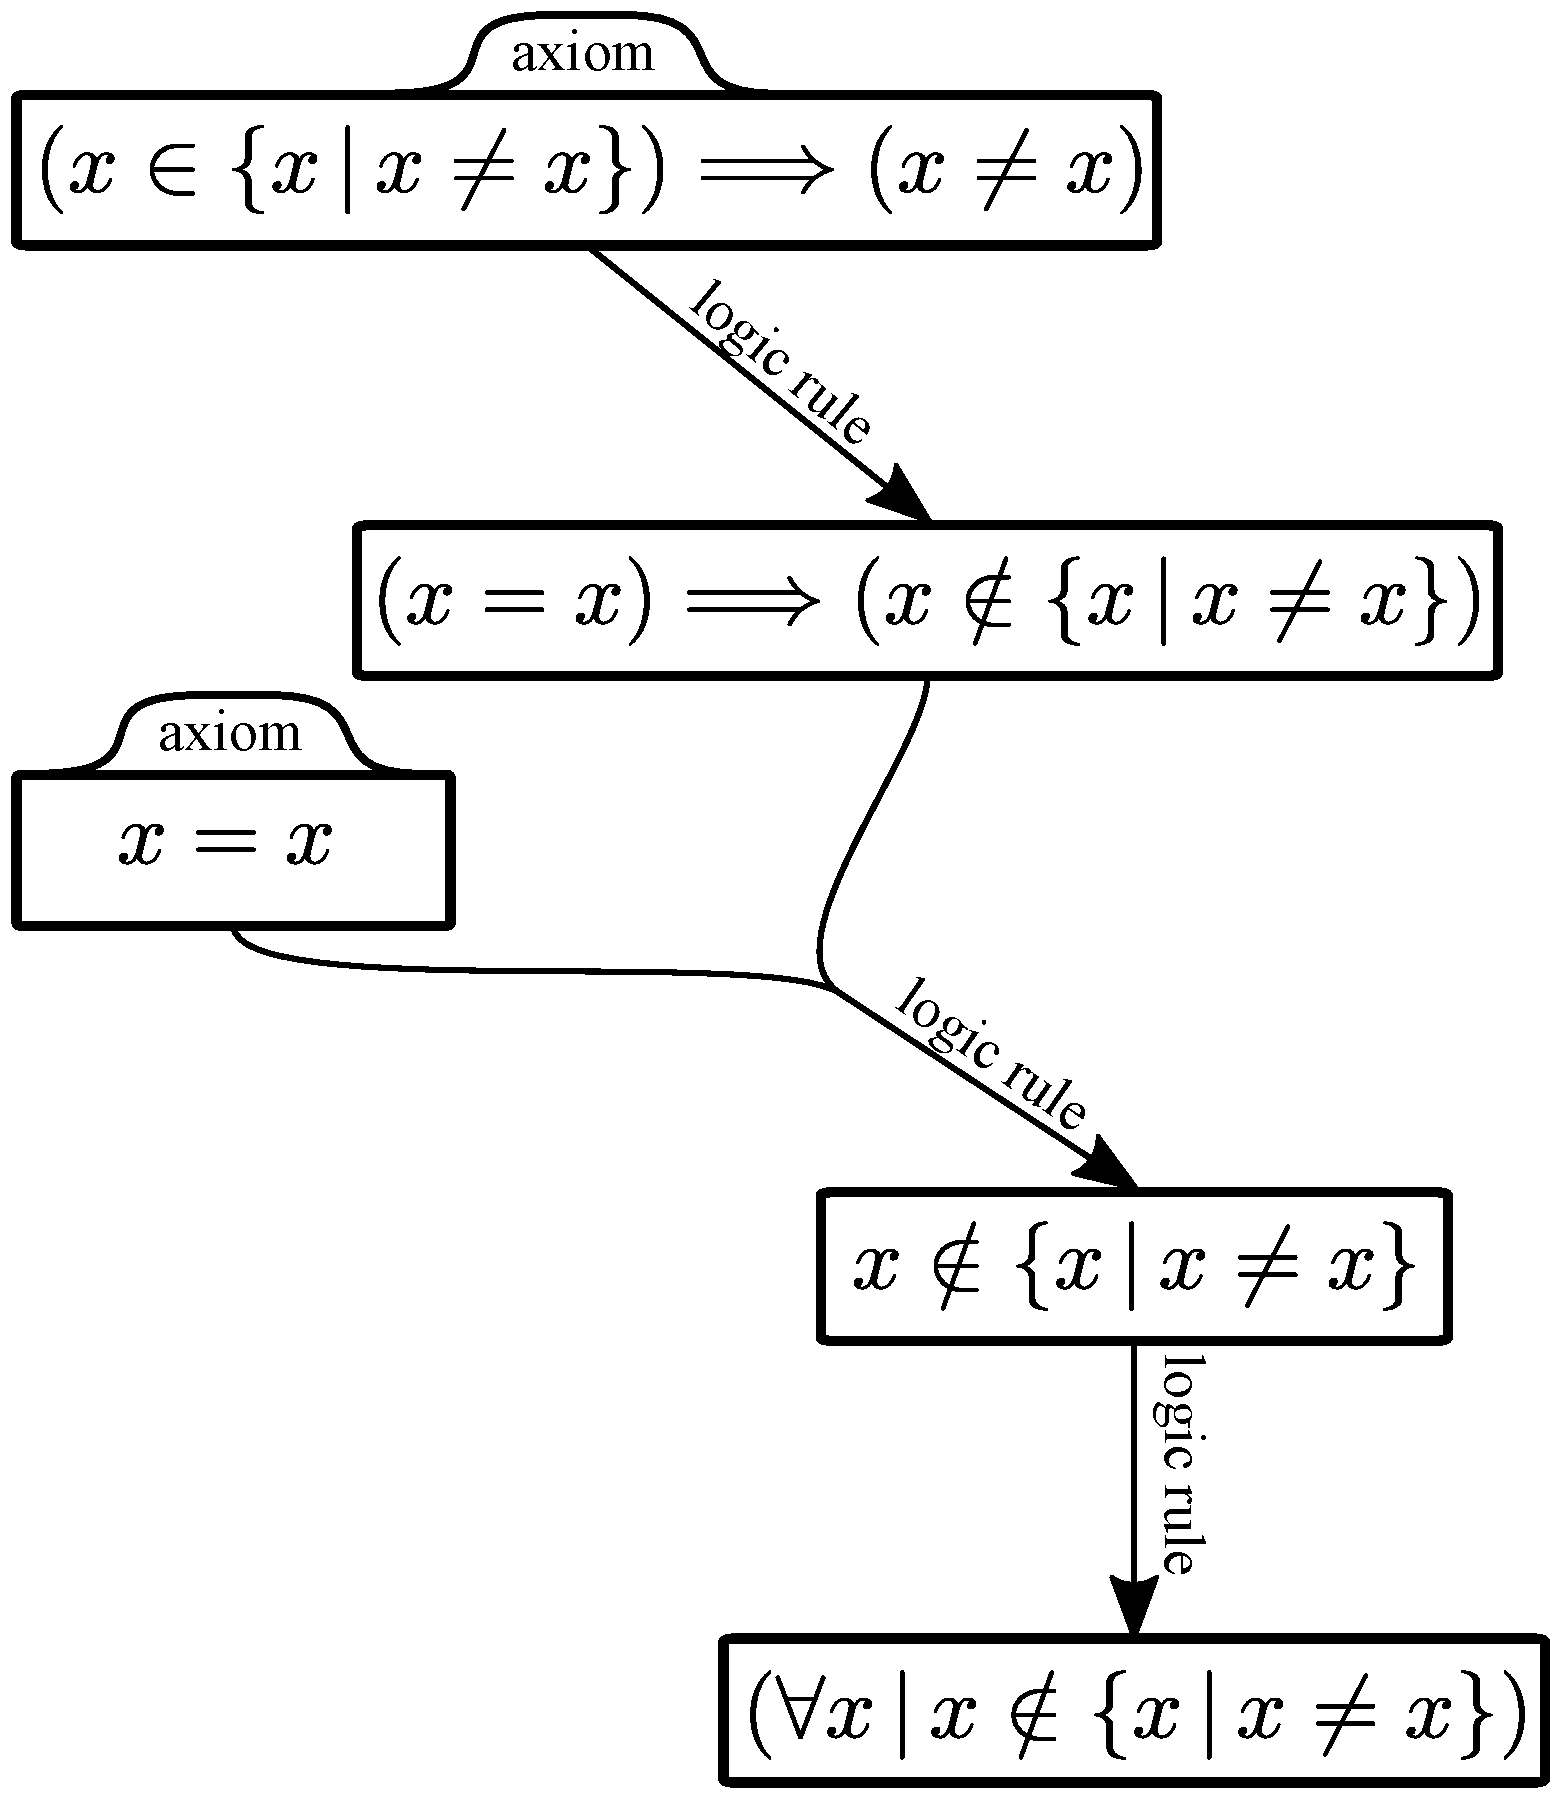
\includegraphics[scale=0.25]{proofFlow.pdf}
\end{center}
Again, don't worry yet about understanding why this works.
What I want you to take away from this is the general structure:
we have axioms serving as starting propositions, and we use logic to ``flow'' out from
the starting points and prove other propositions.

Given a bunch of axioms to start with, what theorems can we deduce?
To answer this question is to do math.

\paragraph{Remark about Axioms}
Axioms often serve to \emph{give meaning} to symbols.
For example, the axiom $x=x$ (along with some other axioms related to equality)
gives meaning to the symbol ``$=$''.
Without the axiom, we would still be able to form propositions like $a=b$ but we would never be able to
prove anything about them.
Suppose you ``disagree'' with the axiom $x=x$ and instead use some other propositions related to ``$=$'' as axioms.
That's perfectly fine-- you would just be giving a different meaning to the symbol ``$=$'' and it would serve a different purpose in your language.

\paragraph{Math is for Humans}
The five-line proof given above is a \emph{formal proof}-- it is written in pure mathematical language
with absolutely no English.
This is great if you want absolute rigor, but
it is not friendly to read if you are not a computer.
The main purpose of a mathematical proof is for it to convince a human that a theorem is true.
But formal proofs make for really inefficient communication between humans.
Thus we are faced with a trade-off: 
we can sacrifice some rigor to gain efficiency of communication.

\emph{Informal proofs} use a mixture of English and mathematics to make arguments.
For an example, look ahead a few paragraphs for an informal version of the five-line proof above.

We need to find a good balance between rigor and efficient communication.
Finding that balance is one of the great challenges when you first learn how to write proofs.
If we sacrifice too much rigor in an argument, then we can lose confidence in its correctness.
Or worse, we can start to prove false things!
When developing a new mathematical theory, it's generally good to err on the side of being more rigorous.
Then, as the theory develops and common patterns of arguments become routine,
one can slowly relax the rigor in favor of efficiency.

Now you can see what this course is all about.
While it is partly giving you some specific mathematical content like set theory,
this course is mainly about how to communicate proofs in that balanced way-- rigorous, yet informal and efficient.

Here is an informal version of the five-line proof from above.

\THM{The set $\ES$ has no elements.}{
If $\ES$ did have an element, say $x$, then we would have $x\neq x$.
But in fact it is an axiom that $x=x$. Thus $\ES$ cannot have any elements.
}

The arguments are essesntially the same ones that appeared in the five-line formal proof.
But, compared to the formal proof, it's much easier to process the arguments (though I'm still not expecting you to do so just yet).

\newpage 
\def\s{0.25}
\newcommand{\rb}[1]{\raisebox{-0.2em}{#1}}
\ex{
In this exercise we will work with a made-up deductive language which works as follows:
\begin{itemize}
\item Propositions are the only part of speech. The propositions are $3\times 3$ grids in which each square is either blank or contains a dot. Here are three random example propositions:
\begin{center}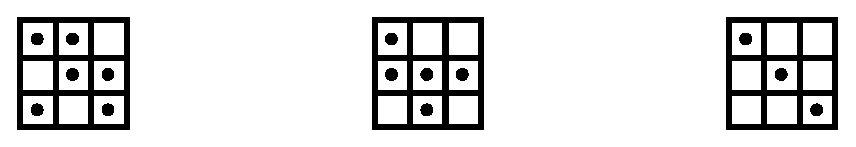
\includegraphics[scale=\s]{gridgame1.pdf}\end{center}
\item There are two logical rules in this language.
The first rule is that if a particular proposition holds, then
its clockwise rotation by ninety degrees follows. So if 
\rb{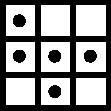
\includegraphics[scale=\s]{gridgame2.pdf}}
holds, then you can deduce that
\rb{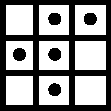
\includegraphics[scale=\s]{gridgame3.pdf}}.
The second rule is that if two propositions $\pA$ and $\pB$ hold, then you can deduce a third proposition
which contains a dot in any square that has a dot in either $\pA$ or $\pB$, but not both.
So for example if you have the two propositions
\rb{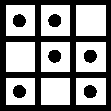
\includegraphics[scale=\s]{gridgame6.pdf}}
and
\rb{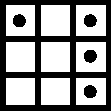
\includegraphics[scale=\s]{gridgame7.pdf}},
then you can deduce from them that
\rb{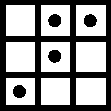
\includegraphics[scale=\s]{gridgame5.pdf}}.
\item There are only two axioms in this language, and they are as follows:
\begin{center}
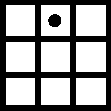
\includegraphics[scale=\s]{gridgame8.pdf}
\hspace{2em}
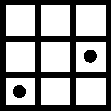
\includegraphics[scale=\s]{gridgame9.pdf}
\end{center}
\end{itemize}
As a demonstration of this deductive language, here is a proof that 
\rb{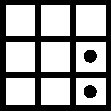
\includegraphics[scale=\s]{gridgame11.pdf}}\ :
\begin{center}
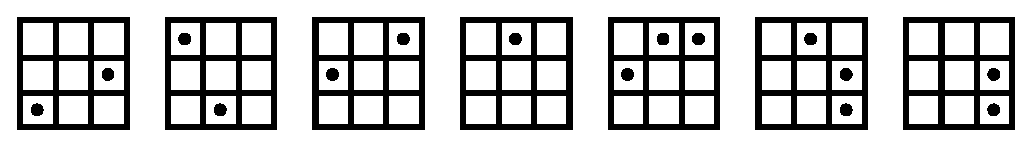
\includegraphics[scale=\s]{gridgame10.pdf}
\end{center}
Can you see how this proof is correct?
These annotations may help:
\begin{center}
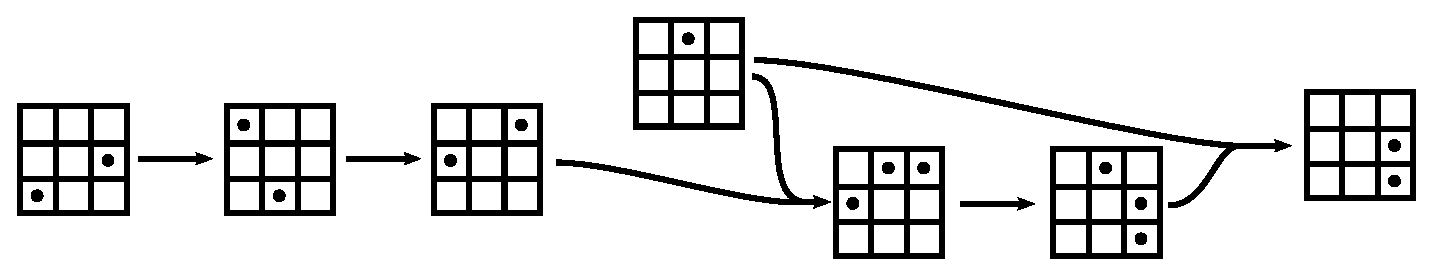
\includegraphics[scale=\s]{gridgame12.pdf}
\end{center}
Now...
\begin{enumerate}
\item
How many propositions are there in this language?
How many propositions do you think there are in mathematics?
How many sentences are there in English?
\item
Give a completely formal proof that 
\rb{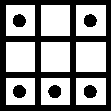
\includegraphics[scale=\s]{gridgame0.pdf}}.
To help out your reader, annotate the proof with arrows like in the example above.
\item (Open-ended) Can you think of a way to write an \emph{informal} version of your proof?
It would be an English description of your proof that does not explain every detail but still captures the essence of your formal proof.
%One way to think of an informal proof is: it somehow gives the reader \emph{instructions} for how to come up with the formal proof.
\item (Irrelevant but fun) Can you figure out how many propositions in this language are provable and how many are not?
\end{enumerate}
}



\subsection{Logic and Writing Mathematical Arguments}

The rest of this course will introduce logic and set theory, starting with logic in this section.
Our goal with logic is not only to understand the rules of deduction,
but also to gain the ability to \emph{write} paragraph-style deductive arguments-- informal proofs.

Logic is all about manipulating \emph{propositions}, so you will not see many \emph{terms} showing up in this section.
In fact, we will find ourselves having to discuss proofs while having nothing in particular to prove anything about.
Mathematical propositions are supposed to say things about mathematical objects;
without any mathematical objects in hand, we cannot form any actual mathematical propositions.
We will proceed with the discussion anyway, using two strategies:

First, we will use capital Greek letters as placeholders for mathematical propositions. Examples include
$$
\pA,
\pB,
\pC,
\pD,
\pE,
\pF.
$$
When you see these capital Greek letters, remember that they are \emph{not variables},
at least not in the sense of mathematical variables. They are not to be replaced by mathematical \emph{objects}.
Rather, they are meant to be replaced by \emph{propositions}.
When they appear in English sentences, they will take the grammatical role of independent clauses.
So, for example, we accept the following as grammatically correct English sentences:
\begin{adjustwidth}{2em}{}
I believe that $\pA$.\\
They thought that $\pA$, but in fact $\pB$.\\
$\pA$.
\end{adjustwidth}

Our second strategy
%for discussing logic without the ability to form mathematical propositions 
is to apply the rules of logic to English sentences.
Even though $\pA$, $\pB$, etc. are supposed to stand for \emph{mathematical} propositions,
we will allow ourselves to replace them by declarative sentences in \emph{English}.
For example, replacing $\pA$ by ``Jim stole the car'' and $\pB$ by ``Jim is an upstanding guy'' in the above examples, we get the sentences
\begin{adjustwidth}{2em}{}
I believe that Jim stole the car.\\
They thought that Jim stole the car, but in fact Jim is an upstanding guy.\\
Jim stole the car.
\end{adjustwidth}
We will stop doing this as soon as we reach section \ref{sec:sets}. At that point, we will start to work with actual mathematical propositions.

\ex{
Which of the following are grammatically correct? Hint: replace Greek letters with English sentences and see what makes sense.
\begin{enumerate}
\item She said that $\pC$, and I think she's onto something.
\item Take that, you accursed $\pA$!
\item Why don't we just $\pB$?
\item To $\pA$, or not to $\pA$, that is the question.
\item Whether $\pC$ or $\pD$, it will always be the case that $\pA$.
\item $\pD$ and $\pF$, but not $\pB$.
\item Despite all the $\pE$, they still wanted to $\pF$.
\item Whenever $\pC$, it turns out that $\pE$.
\item It is not true that $\pA$.
\end{enumerate}
}



\subsubsection{And, Or, and Not}

Given propositions $\pA$ and $\pB$, we can form their \emph{conjunction}
$$
\pA \AND \pB,
$$
which is expressed in English as ``$\pA$ and $\pB$.''
From the conjunction $\pA\AND\pB$, you can deduce $\pA$ and you can deduce $\pB$.
In order to prove that $\pA\AND\pB$, you must prove both that $\pA$ and that $\pB$.
The following diagram, showing what you can deduce from $\pA\AND\pB$, kind of looks like the ``$\AND$'' symbol:
\begin{center}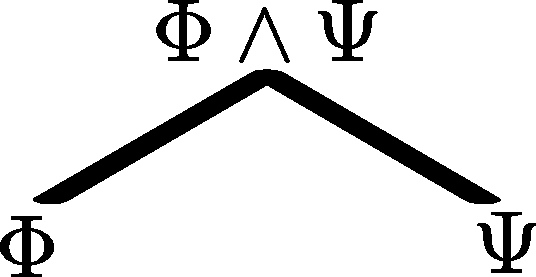
\includegraphics[scale=0.5]{andDiagram.pdf}\end{center}


Given propositions $\pA$ and $\pB$, we can form their \emph{disjunction}
$$
\pA \OR \pB,
$$
which is expressed in English as ``$\pA$ or $\pB$.''
In order to prove that $\pA\OR\pB$, you can either prove that $\pA$ or you can prove that $\pB$.
So if $\pA$ and $\pB$ happen to both hold, then you can still deduce that $\pA\OR\pB$
(unlike the way ``or'' is sometimes used in English).
The following diagram, showing what you can use to deduce $\pA\OR\pB$, kind of looks like the ``$\OR$'' symbol:
\begin{center}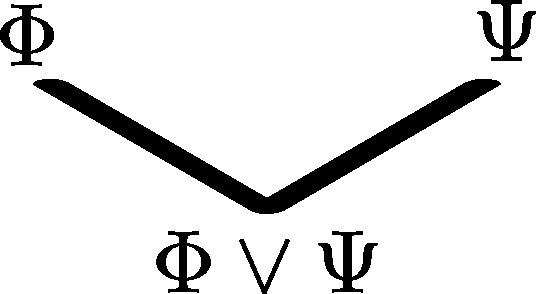
\includegraphics[scale=0.5]{orDiagram.pdf}\end{center}

If you know that $\pA\OR\pB$, then how can you use this fact in your arguments?
You cannot deduce $\pA$ and you cannot deduce $\pB$, so how do you proceed if you want to prove some other proposition $\pC$?
The rule that lets you proceed is called \emph{proof by cases}:
\RULE{Proof by cases}{
Suppose that you can prove $\pC$ by assuming $\pA$, and you can also prove $\pC$ by assuming $\pB$.
Then you can deduce $\pC$ from $\pA\OR\pB$.
}
In a written proof, the format of a proof by cases ends up like this:

\THM{Assuming that either $\pA$ or $\pB$ holds, we have $\pC$.}{
Assume that either $\pA$ or $\pB$ holds.\\
Case 1: Suppose that $\pA$ holds.
\indented{[insert argument here convincing the reader that $\pC$ holds]}
Case 2: Suppose that $\pB$ holds.
\indented{[insert argument here convincing the reader that $\pC$ holds]}
Since $\pC$ holds in both cases, we can conclude that $\pC$ holds.
}

Let's do an example using English sentences.
Suppose you see a plant with three-leaf bunches and you're sure that it's either poison ivy or poison oak, but you don't know which.
Well, you do know that poison ivy is poisonous and that poison oak is poisonous, so you can at least conclude that the plant you see is poisonous, even
if you don't know which type of plant it is.
That's a proof by cases.
To make the proof structure apparent in
the formatting given above, replace $\pA$ by ``the plant is poison ivy,'' replace $\pB$ by ``the plant is poison oak,'' and replace $\pC$ by ``the plant is poisonous.''

%You get something like this:
%\THM{Assuming that the plant is either poison ivy or poison oak, we can conclude that it is poisonous.}{
%Assume that the plant is either poison ivy or poison oak.\\
%Case 1: Suppose the plant is poison ivy.
%\indented{[insert argument convincing the reader that poison ivy is poisonous.]}
%Case 2: Suppose the plant is poison oak.
%\indented{[insert argument convincing the reader that poison oak is poisonous.]}
%Since the plant is poisonous either way, we can conclude that the plant is poisonous.
%}

Given a proposition $\pA$, we can form its \emph{negation}
$$
\neg \pA,
$$
which is expressed in English as ``it is not the case that $\pA$.''
To prove $\neg\pA$ is to disprove $\pA$, and in fact this is what ``disprove'' means.
When $\pA$ holds we say that $\pA$ is \emph{true}, and when $\neg\pA$ holds we say that $\pA$ is \emph{false}.

%It should never be the case that a proposition holds while its negation also holds.
%We hope, at least, that $\pA\AND\not\PA$ is not provable.
A proposition of the form $\pA\AND\neg\pA$ is called a \emph{contradiction}.
If something can both be and not be the case, then our entire deductive system is certainly broken.
We hope that no contradiction is provable in our language.
This leads us to accept the following as a way of proving a negation $\neg\pA$:
%Further, we explicitly deem contradictions to be \emph{impossible}, in the sense that any assumption
%that leads one to deduce a contradiction must be rejected as false.
%In order to prove that $\neg\pA$, you can assume that $\pA$ does hold and then show that this leads to a contradiction.
%This is called a \emph{proof by contradiction}:
\RULE{Proof by contradiction}{
If assuming $\pA$ allows you to deduce a contradiction, then it must be that $\neg\pA$.
}
In a written proof, the format of a proof by contradiction ends up like this:

\THM{$\neg\pA$.}{
Suppose, for the sake of obtaining a contradiction, that $\pA$ holds.
\indented{[insert argument convincing reader that a contradiction, something of the form $\pB\AND\neg\pB$, now follows]}
Since this is a contradiction, we conclude that $\neg\pA$.
}

Let's do an example using English sentences.
Say you're investigating a crime and you are considering a particular suspect.
Assuming the suspect did commit the crime, you can deduce that the suspect must have been at the crime scene on that day.
Upon questioning witnesses, you discover that the suspect was at work and could not have been at the crime scene that day.
This contradiction leads you to reject the original assumption; the suspect must not have committed the crime.
Making an assumption so that you can reject it after deducing an impossible situation-- that is a proof by contradiction.
To make the proof structure apparent in
the formatting given above, replace
$\pA$ by ``the suspect committed the crime'' and replace $\pB$ by ``the suspect was at the crime scene that day''.


The proof by contradiction rule rejects that a mathematical proposition can be both true and false.
There's
another rule involving negation which
enforces that mathematical propositions must be either true or false:
\RULE{Excluded middle}{
$\pA\OR\neg\pA$
}
There is no ``middle ground'' in which a proposition is neither true nor false.






% go back and do a better job presenting rules in terms of  formatting, and separatign susbsections perhaps with illustrated titles



% exercise that helps to understand how in english you can have inclusive and exclusive or, while math is inclusive.

% exercise that shows how parentheses are needed in and-or combinations
% in the same exercise you can show how and distributes over or and vice versa
% maybe the ex can be structured like this: for each of the following deductions, decide whether it is valid or not. if not valid, then justify by... 
  % uhhh truth table? or maybe you can give them some sample true and false english facts to put in, and do an example.

% some kind of exercise involving demorgan's law. or maybe you should write about that above
% idea: a deduction of demorgan's law going one way, and have them prove it going the other way

% maybe an exercise involving truth tables, having them fill one out for basic things and then for more complicated props

\ex{
The ``or'' of mathematical logic sometimes behaves differently from the English ``or.''
Describe a situation in which
\begin{center} ``The cake is flavored with either vanilla or chocolate.'' \end{center}
would pretty much be considered false, while
\begin{center} ``The cake is flavored with vanilla''\ $\OR$\ ``The cake is flavored with chocolate''. \end{center}
would be true.
}




\newcommand{\truthtablefour}[5]{
\begin{tabular}{|c|c|c|}
\hline
$\pA$ & $\pB$ & #1 \\ \hline
F     & F  & #2   \\ \hline
F     & T  & #3   \\ \hline
T     & F  & #4   \\ \hline
T     & T  & #5   \\ \hline
\end{tabular}
}

\newcommand{\truthtabletwo}[3]{
\begin{tabular}{|c|c|}
\hline
$\pA$ & #1 \\ \hline
F     & #2   \\ \hline
T     & #3   \\ \hline
\end{tabular}
}


\def\sp{\hspace{1em}}

\ex{
Thanks to the law of excluded middle, there are only two possibilities for a single proposition $\pA$: it is either true or false.
For \emph{two} propositions $\pA$ and $\pB$, there are \emph{four} possibilities, which we can list in a nice table:
\begin{center}
\begin{tabular}{|c|c|}
\hline
$\pA$ & $\pB$ \\ \hline
F     & F     \\ \hline
F     & T     \\ \hline
T     & F     \\ \hline
T     & T     \\ \hline
\end{tabular}
\end{center}
For three propositions there are eight possibilities, and so on.
This suggests a useful way to think about the logical operators $\AND$, $\OR$, and $\neg$:
\begin{center}
\truthtablefour{$\pA\AND\pB$}{F}{F}{F}{T}
\sp
\truthtablefour{$\pA\OR\pB$}{F}{T}{T}{T}
\sp
\truthtabletwo{$\neg\pA$}{T}{F}
\end{center}
Here we are simply listing all the possibilities for the component propositions $\pA$, $\pB$, etc.,
and then we are indicating whether the complex proposition is true or false in each case. These are called \emph{truth tables}.
\begin{enumerate}
\item
Write out a truth table for $\neg(\pA\AND\pB)$. It should have four rows.

\item
Write out a truth table for $(\pA\AND\pB)\OR\pC$, and also for $\pA\AND(\pB\OR\pC)$.
The table should have eight rows, and you can feel free to make just one table in which 
there is a column for $(\pA\AND\pB)\OR\pC$ and a column for $\pA\AND(\pB\OR\pC)$.

\item
Your answer to the above should convince you that it's a terrible idea to write something like ``$\pA\AND\pB\OR\pC$.''
Replace $\pA$, $\pB$, and $\pC$ by English sentences in $\pA\AND\pB\OR\pC$ such that you get an ambiguous Enlgish sentence.
Explain the ambiguity in your sentence.

\item
Write out a truth table for $(\pA\AND\pB)\AND\pC$, and also for $\pA\AND(\pB\AND\pC)$.
The answer should convince you that there is no trouble at all with writing $\pA\AND\pB\AND\pC$,
though you were probably convinced anyway since $\pA\AND\pB\AND\pC$ can obviously only mean:
``$\pA$, $\pB$, and $\pC$ are all true.''

\item
Write out a truth table for $(\pA\AND\pB)\OR\pA$. This one should just have four rows.
Looking at the table, do you see a way to ``simplify'' the complex proposition  $(\pA\AND\pB)\OR\pA$?

\item
Write out a truth table for $(\pA\AND\pB)\OR\pC$, and also for $(\pA\OR\pC)\AND(\pB\OR\pC)$.
This should show you that $\OR$ can ``distribute'' over $\AND$.

\item
Write out a truth table for $(\pA\OR\pB)\AND\pC$, and also for $(\pA\AND\pC)\OR(\pB\AND\pC)$.
This should show you that $\AND$ can ``distribute'' over $\OR$.
\end{enumerate}
}


\newpage

\note{TODO: Move this exercise to the right place-- I am thinking we should put it later in a derived rules section.}

\ex{
Starting from the assumption $\neg(\pA\AND\pB)$, prove that $(\neg\pA)\OR(\neg\pB)$.
Write your proof using only the logic rules given in this section.
Hints:
The first hint is that excluded middle, proof by contradiction, and proof by cases are all helpful here.
The second hint is to show you the backwards version of what you are being asked to do, just to give you a feeling for the way to write these arguments.
Starting from the assumption $(\neg\pA)\OR(\neg\pB)$, here is a proof that $\neg(\pA\AND\pB)$:
\indented{
Assume $(\neg\pA)\OR(\neg\pB)$.
Suppose, for the sake of contradiction, that $\pA\AND\pB$ holds.
Then $\pA$ holds, and $\pB$ holds. Since we know that $(\neg\pA)\OR(\neg\pB)$ holds, there are two cases to consider:\\[0.5em]
Case 1: Suppose that $\neg\pA$ holds. Then, since we already said that $\pA$ holds, we obtain the contradiction $\pA\AND\neg\pA$.\\[0.5em]
Case 2: Suppose that $\neg\pB$ holds. Then, since we already said that $\pB$ holds, we obtain the contradiction $\pB\AND\neg\pB$.\\[0.5em]
We obtain a contradiction either way, and so we are forced to reject that $\pA\AND\pB$. That is, we have $\neg(\pA\AND\pB)$.
}
}

\note{Here is solution to exercise. IDK what to do with it right now.}

Assume $\neg(\pA\AND\pB)$.
Due to excluded middle, either $\pA$ or $\neg\pA$.\\[0.5em]
Case 1: Suppose that $\pA$ holds. Now if $\pB$ held we would obtain $\pA\AND\pB$, which leads to the contradiction $(\pA\AND\pB)\AND\neg(\pA\AND\pB)$.
Therefore it must be that $\neg\pB$. From this it follows that $\neg\pA\OR\neg\pB$.\\[0.5em]
Case 2: Suppose that $\neg\pA$ holds. Then it immediately follows that $\neg\pA\OR\neg\pB$.\\[0.5em]
Since we ended up with $\neg\pA\OR\neg\pB$ in both cases, we can conclude that $\neg\pA\OR\neg\pB$.

\newpage


\subsubsection{If and Iff}

Given propositions $\pA$ and $\pB$, we can form the \emph{implication}
$$
\pA\ARR\pB,
$$
which is expressed in English as ``if $\pA$, then $\pB$.''
The ``$\pA$'' part of an implication $\pA\ARR\pB$ is called the \emph{hypothesis},
and the ``$\pB$'' part is called the \emph{conclusion}.
To prove $\pA\ARR\pB$,
start by assuming $\pA$ and
then give an argument that $\pB$ follows.
That is, assume the hypotheses and then argue that the conclusion follows.
Such a proof ends up structured like this:

\THM{If $\pA$, then $\pB$.}{
Assume that $\pA$.
\indented{[insert argument convincing reader that $\pB$ holds]}
Thus, $\pA\ARR\pB$.
}

The rule that allows us to use $\pA\ARR\pB$ is modus ponens:
\RULE{Modus ponens}{
Given $\pA\ARR\pB$ and $\pA$, you can deduce $\pB$.
}
Here is also another great rule for using an implication (this one can be derived from modus ponens via a proof by contradiction):
\DRULE{Modus tollens}{
Given $\pA\ARR\pB$ and $\neg\pB$, you can deduce $\neg\pA$.
}

Given  propositions $\pA$ and $\pB$, we can form the \emph{logical equivalence}
$$
\pA\DARR\pB,
$$
which is expressed in English as ``$\pA$ if and only if $\pB$,'' often shortened to ``$\pA$ iff $\pB$.''

An equivalence holds when two propositions are forced to be true or false \emph{together}--
that is, when they are either both true or both false.

To prove an equivalence $\pA\DARR\pB$, simply prove both of the implications $\pA\ARR\pB$ and $\pB\ARR\pA$.
The proof will be structured like this:

\THM{$\pA\DARR\pB$.}{
Assume that $\pA$.
\indented{[insert argument convincing reader that $\pB$ holds]}
Now assume that $\pB$.
\indented{[insert argument convincing reader that $\pA$ holds]}
}

Using an equivalence works a lot like modus ponens, except it goes in both directions.
If you know that $\pA\DARR\pB$, then you can deduce $\pA$ from $\pB$, $\neg\pA$ from $\neg\pB$,
$\pB$ from $\pA$, and $\neg\pB$ from $\neg\pA$.



\def\sp{\hspace{1em}}

Here are the truth tables for $\ARR$ and $\DARR$:
\begin{center}
\truthtablefour{$\pA\ARR\pB$}{???}{???}{F}{T}
\sp
\truthtablefour{$\pA\DARR\pB$}{T}{F}{F}{T}
\end{center}
There should be nothing surprising there, except that I've left some question marks in position where I think you might be surprised.
If $\pA$ is false, then what of the proposition $\pA\ARR\pB$?
It has to be either true or false (excluded middle), so which is it?
Put another way: Suppose you say ``If $3$ is even, then $3$ is divisible by $2$.''
Knowing that $3$ is not even, are you a liar? Is your statement true or false?
The answer is that it's \emph{true}!
Here is the completed truth table for $\ARR$:
\begin{center}
\truthtablefour{$\pA\ARR\pB$}{T}{T}{F}{T}
\end{center}
Putting T there is not an arbitrary choice-- if you agreed with all the previous logical rules then you \emph{must} agree
that $\pA\ARR\pB$ is \emph{true} when $\pA$ is false.
Let me try and convince you. First we need to revisit contradictions.


\def\vsp{\\[0.5em]}

Recall how \emph{proof by contradiction} works:
If an assumption leads to a contradiction, then the assumption is rejected as false.
If you assume $\pB$, and then after some argumentation you deduce $\pA\AND\neg\pA$, then
you can back out of your original assumption and conclude without a doubt that $\neg\pB$.
Now let's think, hypothetically, what would happen if a contradiction $\pA\AND\neg\pA$ were actually \emph{true}?
If $\pA\AND\neg\pA$ holds, then we can prove $\pB$ by contradiciton as follows:
\indented{
Suppose, for the sake of contradiction, that $\neg\pB$ holds.\vsp
Since $\pA\AND\neg\pA$ has already been assumed to hold, we've already reached a contradiction.\vsp
We conclude that $\neg\neg\pB$, and therefore $\pB$, must hold.
}
Let's be clear about what just happened: from the assumption $\pA\AND\neg\pA$, we were able to prove an \emph{arbitrary proposition}!
This mechanism was always present in the proof by contradiction rule, but it is worth highlighting:

\DRULE{Contradictions are powerful!}{
From $\pA\AND\neg\pA$ you can deduce \emph{any} proposition $\pB$.
}

Now back to the question of how to treat $\pA\ARR\pB$ when $\pA$ is false.
Recall that in order to prove $\pA\ARR\pB$, one can assume $\pA$ and then deduce $\pB$.
If we know that $\pA$ is false to start with, then here is a proof that $\pA\ARR\pB$:
\indented{
Assume $\pA$.\vsp
Since $\pA$ is known to be false, we now have a contradiction $\pA\AND\neg\pA$.\vsp
Using ``contradictions are powerful,'' we can now deduce anything we want! In particular, we can deduce $\pB$.
}
Thus if you accept proofs by contradiction as valid, then you must accept that $\pA\ARR\pB$ is true when $\pA$ is false.
An implication that is true because its hypothesis is false is sometimes said to be \emph{vacuously true}.




% use jacoby notes as a guide, but also look at ``thinking about logic'', and also show a truth table and point out the weird part.
% pull out my old psychology course final paper as well


% double neg somewhere in here

% in an exercise: the iff for the version of demorgan's law that you didn't do in prev sec

\subsubsection{Universal and Existential Quantifiers}


% run through the rules and some useful derived rules of logic
% the focus is not formal derivation, but rather to make the rules intuitive and to examine how they influence *writing*
% where truth tables can help make rules intuitive, bring them in. otherwise truth tables are not a main focus
% a section on and,or,not,implies,iff,forall,exists.
% for each:
  %what it makes prop mean. 
  %what you get from having it and how to write that.
  %how to prove it and how to write that.
  %example using english props
  %useful ways it interacts with previous ones.
  %exercises

% don't forget about excluded middle and other such rules... where do those go?


% a comment (maybe put this earlier) on how repetitiveness is okay for now, and better to fix it later. perhaps sian comments on how fix


\section{Set Theory} % and still writing though...
\label{sec:sets}


% develop set theory along the lines of jacoby notes

% some milestones to reach: relations, functions, induction, recursion, natural numbers

% appendix: put some sample well written proofs and badly written proofs




\end{document}



